\Class{Wizard}
{So what if the land becomes barren? It's not like we're going to stick around.}{Datuu Dawnchaser, elf defiler}

Athasian wizards drain energy from the surrounding soil. The method used labels the wizard as a defiler or a preserver. Preservers have the self-control to gather energy without destroying plants. Those who do not, or who feel no remorse about the damage caused, become Defilers. Defilers leave behind sterile soil and infertile ash when they cast spells. Because of this, most wastelanders blame wizards for the desert landscape that dominates the Tablelands today, and their hatred extends to defilers and preservers alike. In the seven cities, arcane magic is outlawed and feared.

Writing is also illegal in the Tablelands, thus wizards have to go to great lengths to conceal their spellbooks, and they have refined this art to the point where even fellow wizards can be hard pressed to identify a spell book. When found, they are precious resources, hoarded and studied by wizards thirsty for knowledge or power.

\SpellcasterTable{3mm}{The Wizard}{
\SpellHeader{9} \\
1st  & +0     & +0 & +0 & +2  & Path, summon familiar, \feat{Scribe Scroll} & 3 & 1 &&&&&&&&\\
2nd  & +1     & +0 & +0 & +3  &            & 4 & 2 &&&&&&&&\\
3rd  & +1     & +1 & +1 & +3  &            & 4 & 2 & 1 &&&&&&&\\
4th  & +2     & +1 & +1 & +4  &            & 4 & 3 & 2 &&&&&&&\\
5th  & +2     & +1 & +1 & +4  & Bonus feat & 4 & 3 & 2 & 1 &&&&&&\\
6th  & +3     & +2 & +2 & +5  &            & 4 & 3 & 3 & 2 &&&&&&\\
7th  & +3     & +2 & +2 & +5  &            & 4 & 4 & 3 & 2 & 1 &&&&&\\
8th  & +4     & +2 & +2 & +6  &            & 4 & 4 & 3 & 3 & 2 &&&&&\\
9th  & +4     & +3 & +3 & +6  &            & 4 & 4 & 4 & 3 & 2 & 1 &&&&\\
10th & +5     & +3 & +3 & +7  & Bonus feat & 4 & 4 & 4 & 3 & 3 & 2 &&&&\\
11th & +5     & +3 & +3 & +7  &            & 4 & 4 & 4 & 4 & 3 & 2 & 1 &&&\\
12th & +6/+1  & +4 & +4 & +8  &            & 4 & 4 & 4 & 4 & 3 & 3 & 2 &&&\\
13th & +6/+1  & +4 & +4 & +8  &            & 4 & 4 & 4 & 4 & 4 & 3 & 2 & 1 &&\\
14th & +7/+2  & +4 & +4 & +9  &            & 4 & 4 & 4 & 4 & 4 & 3 & 3 & 2 &&\\
15th & +7/+2  & +5 & +5 & +9  & Bonus feat & 4 & 4 & 4 & 4 & 4 & 4 & 3 & 2 & 1 &\\
16th & +8/+3  & +5 & +5 & +10 &            & 4 & 4 & 4 & 4 & 4 & 4 & 3 & 3 & 2 &\\
17th & +8/+3  & +5 & +5 & +10 &            & 4 & 4 & 4 & 4 & 4 & 4 & 4 & 3 & 2 & 1\\
18th & +9/+4  & +6 & +6 & +11 &            & 4 & 4 & 4 & 4 & 4 & 4 & 4 & 3 & 3 & 2\\
19th & +9/+4  & +6 & +6 & +11 &            & 4 & 4 & 4 & 4 & 4 & 4 & 4 & 4 & 3 & 3\\
20th & +10/+5 & +6 & +6 & +12 & Bonus feat & 4 & 4 & 4 & 4 & 4 & 4 & 4 & 4 & 4 & 4
}

\subsection{Making a Wizard}
The wizard's greatest strength is also his greatest liability. Often wizards will conceal their abilities, learning to mask their spellcasting behind other actions. For all but the most powerful wizards, secrecy is of prime importance, and some will not exercise their power in the presence of those that they do not feel they can trust. Because of this, and because of their generally frail nature, wizards can often be seen as a liability by those not aware of the power they hide.

\textbf{Races:} Elves and humans are the most likely to be wizards. Elves are more tolerant of the faults of magic, even at its worst, due to their nomadic nature. Defiling simply isn't as much of a concern if the ruined land is fifty miles behind you by the end of the next day. The solitary life lead by most half-elves makes it easier for them to conceal their wizardry, should they choose to follow that path. Some rare halflings and pterrans will take up the arts of wizardry, but these races are so closely tuned to flow of life on Athas that they will never willingly defile. Half-giants, trusting and slow-witted, rarely become wizards, and those that do rarely survive for long. Dwarves rarely take to the magic arts, though their focus allows those that do to become exceptionally skilled. Thri-kreen and muls almost never become wizards.

\textbf{Alignment:} Overall, most wizards display a tendency towards lawfulness. The self-control and restraint necessary to keep oneself secret, as well as the disciplined need for long days of studying take their toll on many of the less careful wizards. Most wizards of good alignment have developed the skill and control necessary to master preserving, and only in the direst of situations would a good-aligned wizard defile. Neutral or evil wizards, however, are more likely to become defilers, though evil preservers are not unheard of.

\subsection{Game Rule Information}

\textbf{Alignment:} Preservers can be of any alignment. Defilers must be of any nongood.

\textbf{Hit Die:} d4.

\subsubsection{Class Skills}
\skill{Bluff} (Cha), \skill{Concentration} (Con), \skill{Craft} (Int), \skill{Decipher Script} (Int), \skill{Disguise} (Cha), \skill{Knowledge} (all skills, taken individually) (Int), \skill{Literacy} (N/A), \skill{Profession} (Wis), and \skill{Spellcraft} (Int).

\textbf{Skill Points per Level:} 2 + Int modifier ($\times4$ at 1st level).

\begin{figure}[t!]
\centering
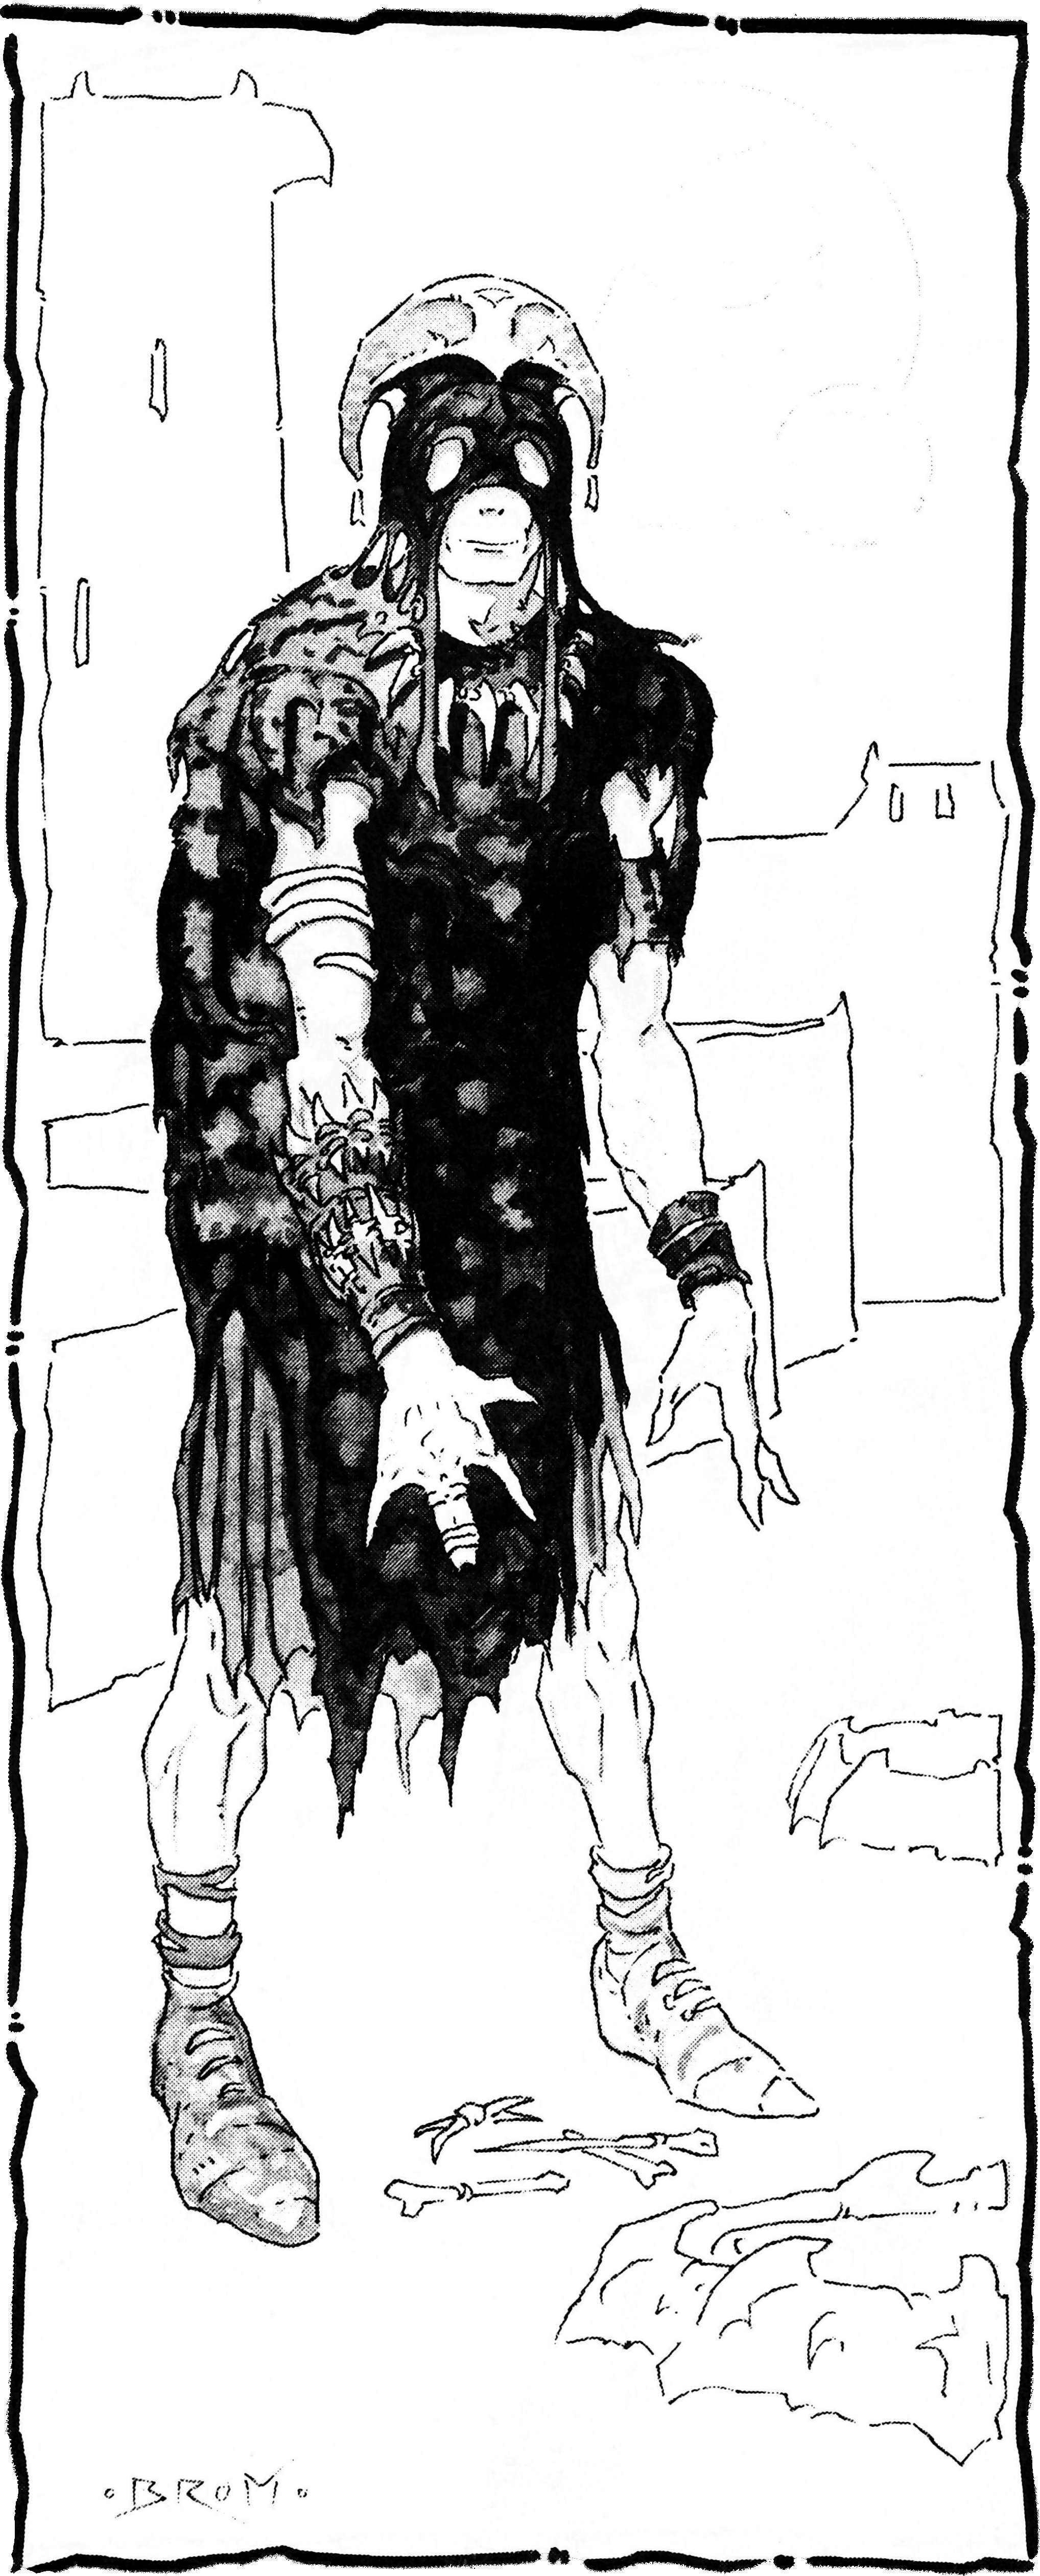
\includegraphics[width=\columnwidth]{images/wiz-1.png}
\WOTC
\end{figure}

\subsubsection{Class Features}
\textbf{Weapon and Armor Proficiency:} Wizards are proficient with the club, dagger, heavy crossbow, light crossbow, and quarterstaff, but not with any type of armor or shield. Armor of any type interferes with a wizard's movements, which can cause her spells with somatic components to fail.

\textbf{Spells:} A wizard casts arcane spells which are drawn from the wizard spell list. A wizard must choose and prepare her spells ahead of time (see below).

To learn, prepare, or cast a spell, the wizard must have an Intelligence score equal to at least 10 + the spell level. The Difficulty Class for a saving throw against a wizard's spell is 10 + the spell level + the wizard's Intelligence modifier.

Like other spellcasters, a wizard can cast only a certain number of spells of each spell level per day. Her base daily spell allotment is given on \tabref{The Wizard}. In addition, she receives bonus spells per day if she has a high Intelligence score.

A wizard may know any number of spells. She must choose and prepare her spells ahead of time by getting a good night's sleep and spending 1 hour studying her spellbook. While studying, the wizard decides which spells to prepare.

% \begin{figure*}[b!]
% \centering
% 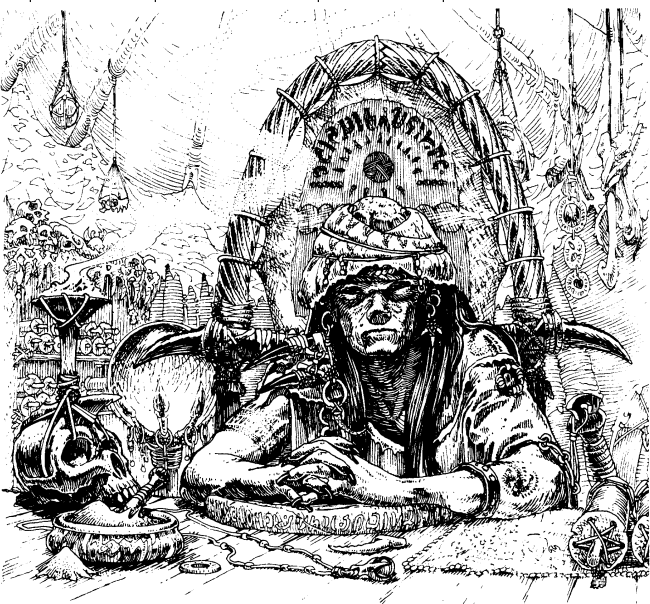
\includegraphics[width=\textwidth-2cm]{images/wizard-5.png}
% \WOTC
% \end{figure*}

\textbf{Bonus Languages:} A wizard may substitute Draconic for one of the bonus languages available to the character because of her race.

\textbf{Familiar:} A wizard can obtain a familiar. Doing so takes 24 hours and uses up magical materials that cost 100 ceramic pieces. A familiar is a magical beast that resembles a small animal and is unusually tough and intelligent. The creature serves as a companion and servant.

The wizard chooses the kind of familiar he gets. As the wizard advances in level, his familiar also increases in power.

If the familiar dies or is dismissed by the wizard, the wizard must attempt a DC 15 Fortitude saving throw. Failure means he loses 200 experience points per wizard level; success reduces the loss to one-half that amount. However, a wizard's experience point total can never go below 0 as the result of a familiar's demise or dismissal. A slain or dismissed familiar cannot be replaced for a year and day. A slain familiar can be raised from the dead just as a character can be, and it does not lose a level or a Constitution point when this happy event occurs.

A character with more than one class that grants a familiar may have only one familiar at a time.

\textbf{Scribe Scroll:} At 1st level, a wizard gains \feat{Scribe Scroll} as a bonus feat.

\textbf{Path:} At 1st level, a wizard must choose a philosophical path: preservation or defilement. This choice is not final. Preservers can defile and be corrupted, and defilers can get redemption.

\textit{Path Dexter:} Wizards who take this path are preservers. They master the balance of the arcane, casting spells with no collateral environmental damage.

Preservers learn one spell at each wizard level from abjuration or divination schools. They are drawn to protection and information spells.

\textit{Path Sinister:} This path is allowed only for nongood wizards. The wizards who take this path are defilers. With every spell cast, defilers take the life out of the plants and soil around them.

Defilers learn one spell at each wizard level from evocation or necromancy schools. They best utilize those darker and more destructive schools.

\textbf{Bonus Feats:} At 5th, 10th, 15th, and 20th level, a wizard gains a bonus feat. At each such opportunity, she can choose a metamagic feat, a raze feat, an item creation feat, or \feat{Spell Mastery}. The wizard must still meet all prerequisites for a bonus feat, including caster level minimums.

These bonus feats are in addition to the feat that a character of any class gets from advancing levels. The wizard is not limited to the categories of item creation feats, metamagic feats, or \feat{Spell Mastery} when choosing these feats.

\textbf{Spellbooks:} A wizard must study her spellbook each day to prepare her spells. She cannot prepare any spell not recorded in her spellbook, except for read magic, which all wizards can prepare from memory.

A wizard begins play with a spellbook containing all 0-level wizard spells (except those from her prohibited school or schools, if any; see School Specialization, below) plus three 1st-level spells of your choice. For each point of Intelligence bonus the wizard has, the spellbook holds one additional 1st-level spell of your choice.

At each new wizard level, she gains three new spells of any spell level or levels that she can cast (based on her new wizard level) for her spellbook, one of which must be from her path's schools. At any time, a wizard can also add spells found in other wizards' spellbooks to her own.

\subsubsection{Familiars}
A familiar is a normal animal that gains new powers and becomes a magical beast when summoned to service by a wizard. It retains the appearance, Hit Dice, base attack bonus, base save bonuses, skills, and feats of the normal animal it once was, but it is treated as a magical beast instead of an animal for the purpose of any effect that depends on its type. Only a normal, unmodified animal may become a familiar. An animal companion cannot also function as a familiar.

A familiar also grants special abilities to its master, as given on the table below. These special abilities apply only when the master and familiar are within 1.5 kilometer of each other.

Levels of different classes that are entitled to familiars stack for the purpose of determining any familiar abilities that depend on the master's level.

\Table{Familiars}{l X}{
	\tableheader Familiar & \tableheader Special\\
	Bat & Master gains a +3 bonus on \skill{Listen} checks\\
	Cat & Master gains a +3 bonus on \skill{Move Silently} checks\\
	Dustgull & Master gains a +3 bonus on \skill{Spot} checks\\
	Hawk & Master gains a +3 bonus on \skill{Spot} checks in bright light\\
	Kes'trekel & Master gains a +2 bonus on Reflex saves\\
	Lizard & Master gains a +3 bonus on \skill{Climb} checks\\
	Owl & Master gains a +3 bonus on \skill{Spot} checks in shadows\\
	Rat & Master gains a +2 bonus on Fortitude saves\\
	Raven$\dagger$ & Master gains a +3 bonus on \skill{Appraise} checks\\
	Skyfish & Master gains a +3 bonus on \skill{Swim} checks\\
	Sygra & Master gains a +3 hit points\\
	Tiny viper & Master gains a +3 bonus on \skill{Bluff} checks\\
	% Toad & Master gains +3 hit points\\
	% Weasel & Master gains a +2 bonus on Reflex saves
	\rowcolor{white}
	\multicolumn{2}{p{\columnwidth}}{$\dagger$ A raven familiar can speak one language of its master's choice as a supernatural ability.}
}


\textbf{Familiar Basics:} Use the basic statistics for a creature of the familiar's kind, but make the following changes:

\textit{Hit Dice:} For the purpose of effects related to number of Hit Dice, use the master's character level or the familiar's normal HD total, whichever is higher.

\textit{Hit Points:} The familiar has one-half the master's total hit points (not including temporary hit points), rounded down, regardless of its actual Hit Dice.

\textit{Attacks:} Use the master's base attack bonus, as calculated from all his classes. Use the familiar's Dexterity or Strength modifier, whichever is greater, to get the familiar's melee attack bonus with natural weapons.

Damage equals that of a normal creature of the familiar's kind.

\textit{Saving Throws:} For each saving throw, use either the familiar's base save bonus (Fortitude +2, Reflex +2, Will +0) or the master's (as calculated from all his classes), whichever is better. The familiar uses its own ability modifiers to saves, and it doesn't share any of the other bonuses that the master might have on saves.

\textit{Skills:} For each skill in which either the master or the familiar has ranks, use either the normal skill ranks for an animal of that type or the master's skill ranks, whichever are better. In either case, the familiar uses its own ability modifiers. Regardless of a familiar's total skill modifiers, some skills may remain beyond the familiar's ability to use.

\Table{Familiar Progression}{b{1.4cm} Z{1.2cm} c X}{
	\tableheader Master Class Level & \tableheader Natural Armor Adj. & \tableheader Int & \tableheader Special\\
	1st--2nd & +1 & 6 & Alertness, improved evasion, share spells, empathic link\\
	3rd--4th & +2 & 7 & Deliver touch spells\\
	5th--6th & +3 & 8 & Speak with master\\
	7th--8th & +4 & 9 & Speak with animals of its kind\\
	9th--10th & +5 & 10 & \\
	11th--12th & +6 & 11 & Spell resistance\\
	13th--14th & +7 & 12 & Scry on familiar\\
	15th--16th & +8 & 13 & \\
	17th--18th & +9 & 14 & \\
	19th--20th & +10 & 15 &
}

\textbf{Familiar Ability Descriptions:} All familiars have special abilities (or impart abilities to their masters) depending on the master's combined level in classes that grant familiars, as shown on the table above. The abilities given on the table are cumulative.

\textit{Natural Armor Adj.:} The number noted here is an improvement to the familiar's existing natural armor bonus.

\textit{Int:} The familiar's Intelligence score.

\textit{Alertness (Ex):} While a familiar is within arm's reach, the master gains the \feat{Alertness} feat.

\textit{Improved Evasion (Ex):} When subjected to an attack that normally allows a Reflex saving throw for half damage, a familiar takes no damage if it makes a successful saving throw and half damage even if the saving throw fails.

\textit{Share Spells:} At the master's option, he may have any spell (but not any spell-like ability) he casts on himself also affect his familiar. The familiar must be within 1.5 meter at the time of casting to receive the benefit.

If the spell or effect has a duration other than instantaneous, it stops affecting the familiar if it moves farther than 1.5 meter away and will not affect the familiar again even if it returns to the master before the duration expires. Additionally, the master may cast a spell with a target of ``You'' on his familiar (as a touch range spell) instead of on himself.

A master and his familiar can share spells even if the spells normally do not affect creatures of the familiar's type (magical beast).

\textit{Empathic Link (Su):} The master has an empathic link with his familiar out to a distance of up to 1.5 kilometer. The master cannot see through the familiar's eyes, but they can communicate empathically. Because of the limited nature of the link, only general emotional content can be communicated.

Because of this empathic link, the master has the same connection to an item or place that his familiar does.

\textit{Deliver Touch Spells (Su):} If the master is 3rd level or higher, a familiar can deliver touch spells for him. If the master and the familiar are in contact at the time the master casts a touch spell, he can designate his familiar as the ``toucher.'' The familiar can then deliver the touch spell just as the master could. As usual, if the master casts another spell before the touch is delivered, the touch spell dissipates.

\textit{Speak with Master (Ex):} If the master is 5th level or higher, a familiar and the master can communicate verbally as if they were using a common language. Other creatures do not understand the communication without magical help.

\textit{Speak with Animals of Its Kind (Ex):} If the master is 7th level or higher, a familiar can communicate with animals of approximately the same kind as itself (including dire varieties): bats with bats, rats with rodents, cats with felines, hawks and owls and ravens with birds, lizards and snakes with reptiles, toads with amphibians, weasels with similar creatures (weasels, minks, polecats, ermines, skunks, wolverines, and badgers). Such communication is limited by the intelligence of the conversing creatures.

\textit{Spell Resistance (Ex):} If the master is 11th level or higher, a familiar gains spell resistance equal to the master's level + 5. To affect the familiar with a spell, another spellcaster must get a result on a caster level check (1d20 + caster level) that equals or exceeds the familiar's spell resistance.

\textit{Scry on Familiar (Sp):} If the master is 13th level or higher, he may scry on his familiar (as if casting the scrying spell) once per day.

\begin{figure}[b!]
\centering
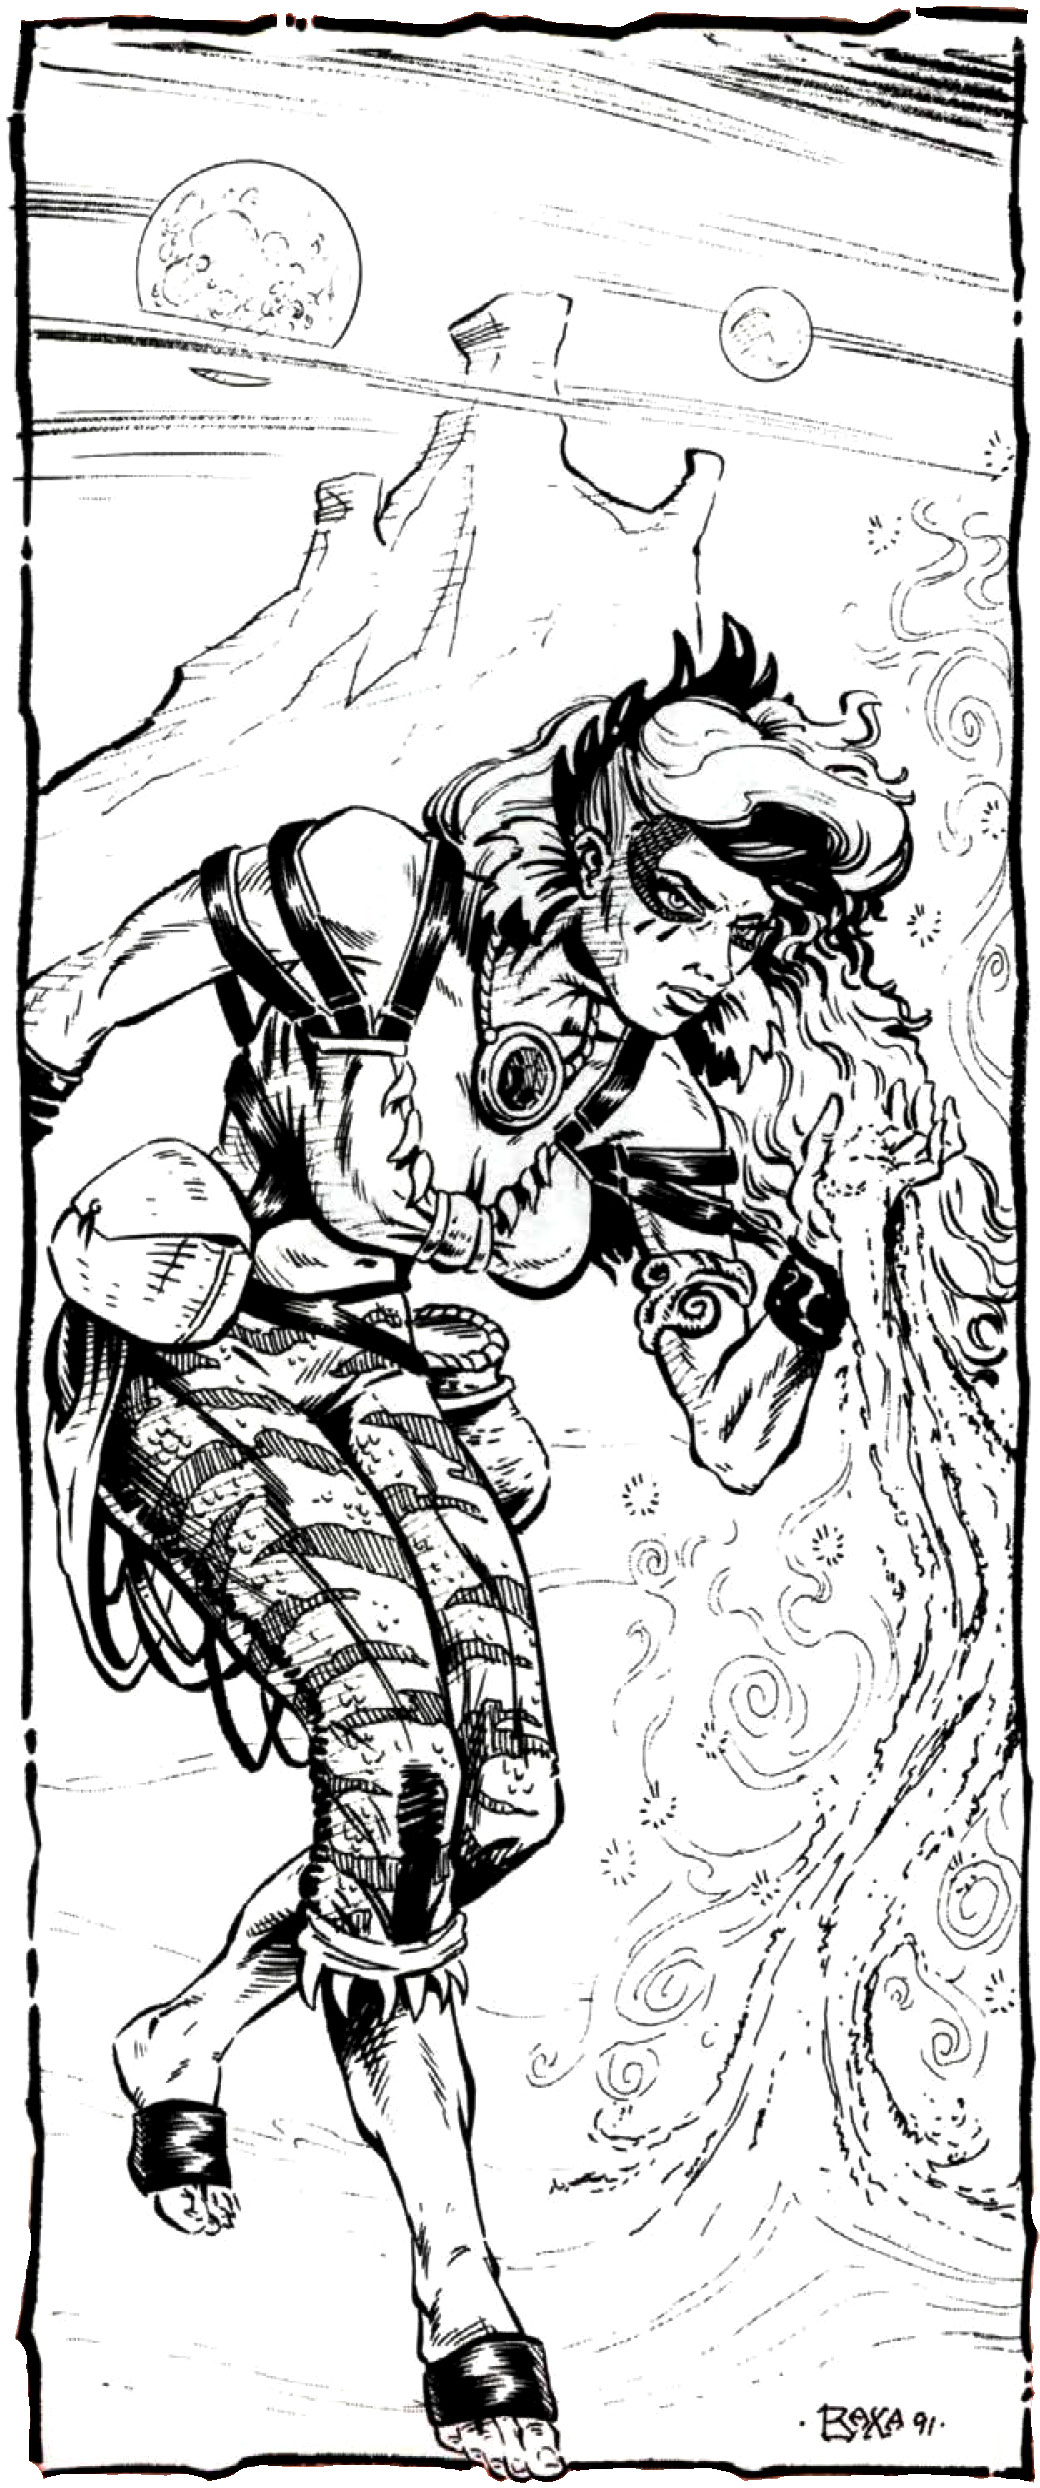
\includegraphics[width=\columnwidth]{images/wizard-2.png}
\WOTC
\end{figure}

\subsubsection{School Specialization}
A school is one of eight groupings of spells, each defined by a common theme. If desired, a wizard may specialize in one school of magic (see below). Specialization allows a wizard to cast extra spells from her chosen school, but she then never learns to cast spells from some other schools.

A specialist wizard can prepare one additional spell of her specialty school per spell level each day. She also gains a +2 bonus on \skill{Spellcraft} checks to learn the spells of her chosen school.

The wizard must choose whether to specialize and, if she does so, choose her specialty at 1st level. At this time, she must also give up two other schools of magic (unless she chooses to specialize in divination; see below), which become her prohibited schools.

A wizard can never give up divination to fulfill this requirement.

Spells of the prohibited school or schools are not available to the wizard, and she can't even cast such spells from scrolls or fire them from wands. She may not change either her specialization or her prohibited schools later.

The eight schools of arcane magic are abjuration, conjuration, divination, enchantment, evocation, illusion, necromancy, and transmutation.

Spells that do not fall into any of these schools are called universal spells.


\textbf{Abjuration:} Spells that protect, block, or banish. An abjuration specialist is called an abjurer.

\textbf{Conjuration:} Spells that bring creatures or materials to the caster. A conjuration specialist is called a conjurer.

\textbf{Divination:} Spells that reveal information. A divination specialist is called a diviner. Unlike the other specialists, a diviner must give up only one other school.

\textbf{Enchantment:} Spells that imbue the recipient with some property or grant the caster power over another being. An enchantment specialist is called an enchanter.

\textbf{Evocation:} Spells that manipulate energy or create something from nothing. An evocation specialist is called an evoker.

\textbf{Illusion:} Spells that alter perception or create false images. An illusion specialist is called an illusionist.

\textbf{Necromancy:} Spells that manipulate, create, or destroy life or life force. A necromancy specialist is called a necromancer.

\textbf{Transmutation:} Spells that transform the recipient physically or change its properties in a more subtle way. A transmutation specialist is called a transmuter.

\textbf{Universal:} Not a school, but a category for spells that all wizards can learn. A wizard cannot select universal as a specialty school or as a prohibited school. Only a limited number of spells fall into this category.

\subsubsection{Ex-Defilers}
Arcane casters who defile must roll a Will save DC 10 + spell level + amount of times previously defiled. Failing this save, they become defilers. Preservers succeeding the save lose their preserver status and become tainted. For more rules on defiling, see \chapref{Magic}.

Tainted wizards are not defilers, but risk becoming so. Tainted wizards may seek redemption from a druid. The druid, if willing and able, can cast a \spell{conversion} spell on the tainted wizard, restoring her preserver status (reset the number of times defiled to zero). The wizard loses 100 XP per arcane spellcaster level.

Defilers can also seek redemption, but lose 1,000 XP per arcane spellcaster level. Usually the defiler must undertake a quest or otherwise demonstrate a true willingness to redeem herself before the druid casts the \spell{conversion} spell.


\subsection{Playing a Wizard}
You are a master of arcane secrets. You have learned, either on your own, or from someone in your family, how to draw on vegetable life in order to power your spells. But such power comes with a caveat, arcane magic is universally feared and hated. You might be inclined to see conspiracies and enemies where none exist, so accustomed are you to being hunted and persecuted by the general populace and sorcerer-king's templars because of your talents.

Mostly, you adventure to perfect your understanding and mastery of magic. You likely prefer endeavors that allow frequent use of your abilities, or those that promise access to ancient lore. You might have personal goals as well, and it's not uncommon for an Athasian wizard to adventure for the sake of riches, power, eternal life, or any other ``standard'' adventurer motive.

\subsubsection{Religion}
Wizards frequently find themselves at odds with the elemental forces that grant clerics their powers, though it is not unheard of for preservers to forge an Elemental Pact. Some preservers might also associate themselves with the assorted Spirits of the Land. Since they understand the sorcerer-kings to simply be exceptionally advanced wizards, they are not given to revering their kings, as some of their more naive brothers are known to do.

\subsubsection{Other Classes}
Wizards have a difficult time relating to most of the other classes. Templars and wizards are, in most cases, deadly enemies across an irreconcilable gap---the exception is those rare defilers in the employ of the sorcerer-kings. Likewise, druids are likely to consider any wizard a potential defiler, and would turn on a companion the moment this suspicion is confirmed. Due to their similar, ``underground'' nature, wizards feel a certain respect for bards. While preservers enjoy an uneasy truce with the elemental powers, defilers and paraelemental clerics tend get along quite well.

\subsubsection{Combat}
Athasian wizards stay back from melee and use your spells to either destroy your enemies or enhance your companion's abilities. Secrecy is a major component, even more so if you are a defiler. Casting even of the simplest of arcane spells can focus all of your enemies' attention to you, even more so if you are a defiler. Be prepared to run of fly away in such cases.

\subsubsection{Advancement}
Continuing your advancement as a wizard requires a substantial amount of time and effort. You must procure and study arcane texts, not merely to learn new spells, but to comprehend the nature of what you do.

When you not studying, you are practicing, training your mind and your body to channel ever greater amounts of life force.

As you start to progress in the class, consider studying other sources of arcane energy, such as the Black, the Gray, and the Cerulean, since those would remove your dependency on vegetable life around you. Most wizards seek to become some day as powerful as Dragon Kings or the fabled winged creature the Urikite known as Korgunard turned into.

Mechanically, you should increase your Intelligence and Charisma as you attain levels. Beyond this, focus on feats (such as Path Dexter or Path Sinister) and skills that enhance your spells and provide you the abilities you need to remain in secrecy, mainly Bluff and Disguise.


\subsection{Starting Packages}
\subsubsection{The Dexter}
Pterran Wizard

\textbf{Ability Scores:} Str 8, Dex 10, Con 10, Int 15, Wis 16, Cha 15.

\textbf{Skills:} \skill{Bluff}, \skill{Concentration}, \skill{Disguise}, \skill{Knowledge} (arcana), \skill{Knowledge} (local), \skill{Spellcraft}.

\textbf{Languages:} Common, Elven, Saurian.

\textbf{Feat:} \feat{Path Dexter}.

\textbf{Weapons:} Dagger (1d4/19--20, 3 m)

Light crossbow with 20 bolts (1d6/$\times$3, 18 m).

\textbf{Armor:} Padded (+1 AC).

\textbf{Other Gear:} Standard adventurer's kit, spell

component pouch, 31 cp.

\subsubsection{The Concurrent}
Human Wizard

\textbf{Ability Scores:} Str 8, Dex 13, Con 10, Int 15, Wis 14, Cha 12.

\textbf{Skills:} \skill{Bluff}, \skill{Concentration}, \skill{Decipher Script}, \skill{Disguise}, \skill{Knowledge} (arcana), \skill{Knowledge} (local), \skill{Spellcraft}.

\textbf{Languages:} City language, Common, Elven.

\textbf{Feat:} \feat{Alertness}, \feat{Improved Initiative}.

\textbf{Weapons:} Dagger (1d4/19--20, 3 m)

Light crossbow with 20 bolts (1d6/$\times$3, 18 m).

\textbf{Armor:} Padded (+1 AC).

\textbf{Other Gear:} Standard adventurer's kit, spell component pouch, 31 cp.

\subsubsection{The Sinister}
Elf Wizard

\textbf{Ability Scores:} Str 10, Dex 16, Con 10, Int 15, Wis 13, Cha 8.

\textbf{Skills:} \skill{Bluff}, \skill{Concentration}, \skill{Knowledge} (arcana), \skill{Knowledge} (local), \skill{Spellcraft}.

\textbf{Languages:} City language, Common, Elven.

\textbf{Feat:} \feat{Destructive Raze}.

\textbf{Weapons:} Dagger (1d4/19--20, 3 m)

Light crossbow with 20 bolts (1d6/$\times$3, 18 m).

\textbf{Armor:} Padded (+1 AC).

\textbf{Other Gear:} Standard adventurer's kit, spell component pouch, 31 cp.


\subsection{Wizards on Athas}
\Quote{'Witch!' they chanted. 'Kill the witch!' By the time the soldiers woke, the crowd had finished her off, and worse. The mage's death did not satisfy the mob; her body suffered much more. When the mul leader shouted, 'we'll take her and burn her!' they cheered. For the only time in my life I saw a crowd cheer for Kalak's guards. For the first time I saw wizard's magic. For the first time I understood its peril.}{Manok, Tyrian wizard}

On Athas, the energy for wizardly magic doesn't come from some extradimensional source as it does on other worlds, but from the living environment itself. It provides great power to those who can gather and shape it, though the cost to Athas can be beyond measure.

In recent times wizards have emerged who have learned to draw energy from alternate sources that have no impact on the environment, see Prestige Class Appendix I for more information.

\subsubsection{Daily Life}
The kinds of activities that appeal to wizards depend largely on their alignment and energy gathering method. Good wizards spend their time trying to restore the devastation of Athas and fighting against the forces of the sorcerer-kings, while evil preservers of defilers are interested in helping themselves.

When not adventuring, Athasian wizards spend the majority of their time in study and in hiding. Much like wizards from other settings, they must constantly research new spells and study ancient arcane texts so thoroughly that they have little time to devote to other endeavors.

\subsubsection{Notables}
Usually wizards try to stay incognito for as long as they can, since their survival depends on it. However, a few wizards manage to become quite famous on Athas. Royal defilers and arena necromancers, such as Dote Mal Payn, even though hated by the general populace are sponsored by their sorcerer-kings and do not need to hide their skills. Sadira of Tyr was made famous for her contribution in killing King Kalak the Tyrant and the Dragon, and she has become the first (and maybe the only one) wizard able to tap into the power of the crimson sun. The most famous wizards are the Dragon Kings, of course, who can destroy both plant life and living creatures to power their spells.

\subsubsection{Organizations}
Wizardly magic on Athas isn't as codified and formal as it is in other campaign settings. For example, there are no academies or colleges for teaching the wizardly arts. Instead, a wizard-in-training must find a teacher, which isn't very easy in a world where wizards must hide their profession in order to survive. For protection from nearly universal hatred, the good wizards of Athas and their allies have formed secret societies, collectively known as the Veiled Alliance.

However, each city-state holds a different Alliance, they do not cooperate, and they share no leaders. Members of one Alliance do not automatically become members of another. At best, the different groups respect each other, and may offer courtesy assistance to a foreign member who arrives in town.

Defilers don't usually organize together, but they often join organizations, especially Merchant Houses and raiding tribes.

\subsubsection{NPC Reactions}
Arcane magic in Athas is viewed as more dangerous and destructive than helpful, so general NPC attitudes towards someone suspected to be a wizard range from indifferent to unfriendly. If a NPC actually witness a wizard drawing magical energy or casting a spell, the resultant fear and hatred shifts the NPC's attitude toward hostile.

Arcane magic is banned in almost all city-states; Tyr has unbanned it after FY 0 after Kalak was killed and Kurn has no qualms about preserving magic. Templars constantly patrol the streets searching for wizards and arcane items.

\subsubsection{Wizard Lore}

Characters with ranks in \skill{Knowledge} (arcana) can research wizards to learn more about them. When a character makes a skill check, read or paraphrase the following, including the information from lower DCs.

\textbf{DC 10:} Wizards are magic users that fuel their spells with plant life.

\textbf{DC 15:} A wizard can be either a defiler or a preserver. Only the first destroys the land when casting a spell. Defilers can increase the potency of their spells by destructing larger areas of vegetation than necessary.

\textbf{DC 20:} Some say that other wizards have developed a way to draw energy from other source than plants.


% \begin{figure}[b!]
% \centering
% 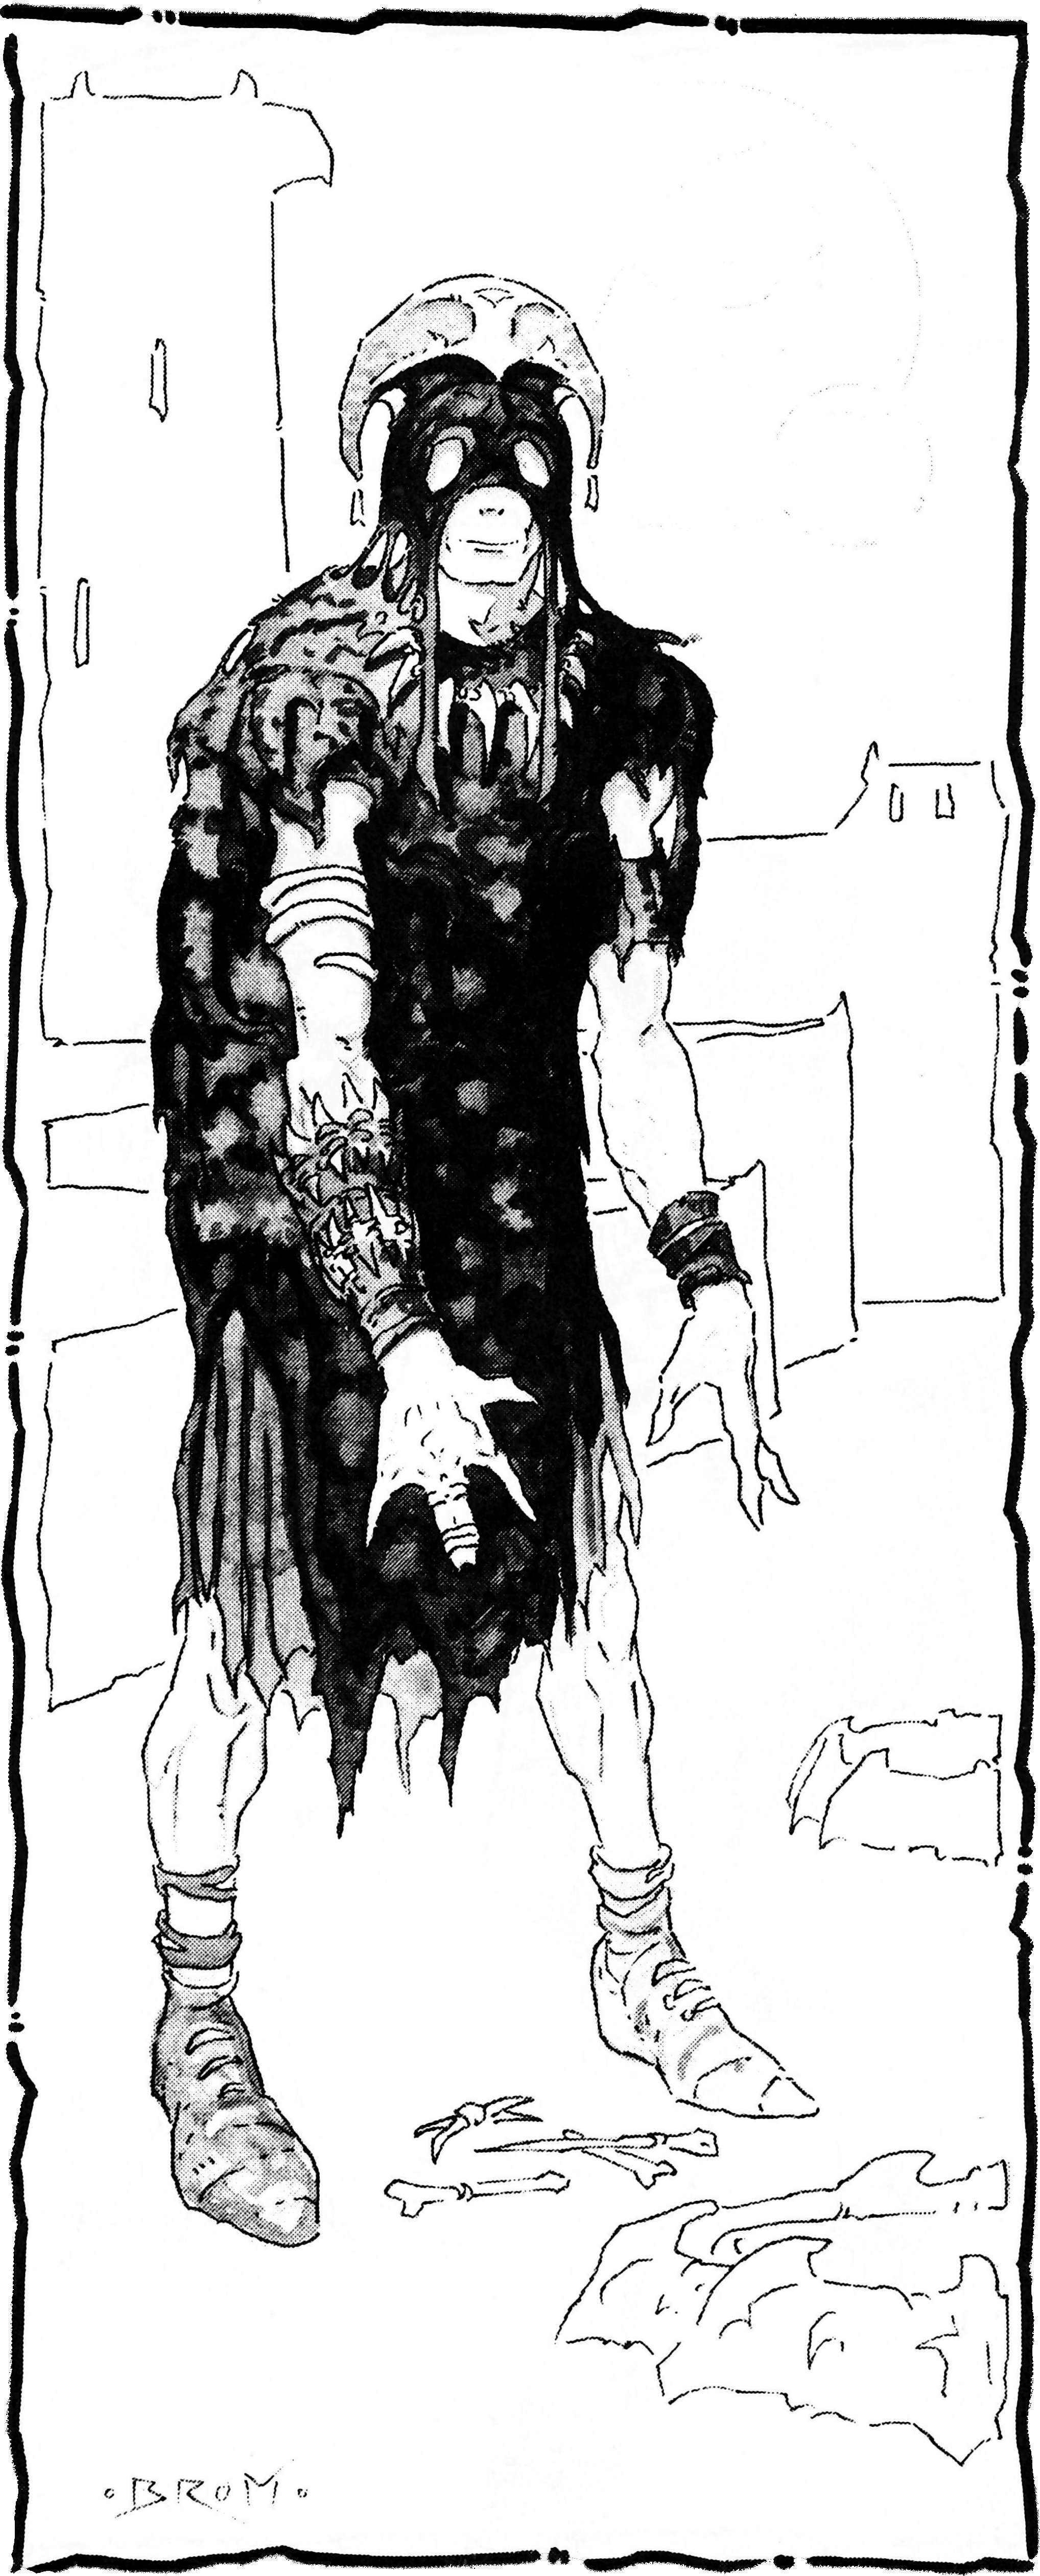
\includegraphics[width=\columnwidth-12mm]{images/wiz-1.png}
% \WOTC
% \end{figure}